\documentclass{article}
\usepackage{comment}
\usepackage{graphicx} % Required for inserting images
\usepackage[compat=1.0.0]{tikz-feynman} % For Feynman diagram drawings 
\usepackage{xcolor}
\title{Feynman Diagrams}
\author{SOUMYA SARKAR}
\date{}

\begin{document}

\section{Simple QED diagrams}
$$e^{+} e^{-} \rightarrow \gamma^{*} \rightarrow e^{+} e^{-}$$

\centering
\begin{tikzpicture}[scale=1.5]
\begin{feynman}

\vertex (i1) at (0,1) {$e^-$};
\vertex (i2) at (0,-1) {$e^+$};

\vertex (a) at (1,0);
\vertex (b) at (2,0);

\vertex (f1) at (3,1) {$e^-$};
\vertex (f2) at (3,-1) {$e^+$};

\diagram*{
  (i1) -- [fermion] (a),
  (i2) -- [anti fermion] (a),
  (a) -- [photon] (b),
  (b) -- [fermion] (f1),
  (b) -- [anti fermion] (f2),
};

\end{feynman}
\end{tikzpicture}

$$e^{-} \gamma \rightarrow e^{-} \rightarrow e^{-} \gamma$$

\begin{tikzpicture}[scale=1.5]
\begin{feynman}

\vertex (i1) at (0,1) {$e^-$};
\vertex (i2) at (0,-1) ;

\vertex (a) at (1,0);
\vertex (b) at (2,0);

\vertex (f1) at (3,1) {$e^-$};
\vertex (f2) at (3,-1) ;

\diagram*{
  (i1) -- [fermion] (a),
  (i2) -- [photon] (a),
  (a) -- [fermion] (b),
  (b) -- [fermion] (f1),
  (b) -- [photon] (f2),
};

\end{feynman}
\end{tikzpicture}

$$e^{+} e^{-} \rightarrow \gamma^{*} \rightarrow e^{+} e^{-}$$ with labels

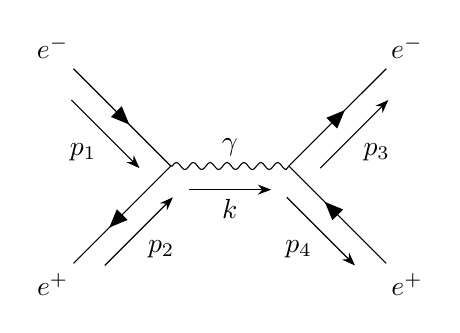
\begin{tikzpicture}[scale=1.5]
\begin{feynman}

\vertex (i1) at (0,1) {$e^-$};
\vertex (i2) at (0,-1) {$e^+$};

\vertex (a) at (1,0);
\vertex (b) at (2,0);

\vertex (f1) at (3,1) {$e^-$};
\vertex (f2) at (3,-1) {$e^+$};

\diagram*{
  (i1) -- [fermion, momentum'={\(p_1\)}] (a),
  (i2) -- [anti fermion, momentum'={\(p_2\)}] (a),
  (a) -- [photon, edge label=\(\gamma\), momentum'={\(k\)}] (b),
  (b) -- [fermion, momentum'={\(p_3\)}] (f1),
  (b) -- [anti fermion, momentum'={\(p_4\)}] (f2),
};

\end{feynman}
\end{tikzpicture}

$\pi^0 \rightarrow \gamma\gamma$ diagram

\begin{tikzpicture}[scale=1.5]
\begin{feynman}

\vertex (i1) at (0,0) {$\pi^0$};

\vertex (a) at (1,0);
\vertex (b) at (2,1);
\vertex (c) at (2,-1);

\vertex (f1) at (3,1);
\vertex (f2) at (3,-1);

\diagram*{
  (i1) -- [scalar] (a),
  (a) -- [] (b),
  (a) -- [] (c),
  (b) -- [] (c),
  
  (b) -- [photon] (f1),
  (c) -- [photon] (f2),
};

\end{feynman}
\end{tikzpicture}

\newpage
\section*{Higgs Diagrams}

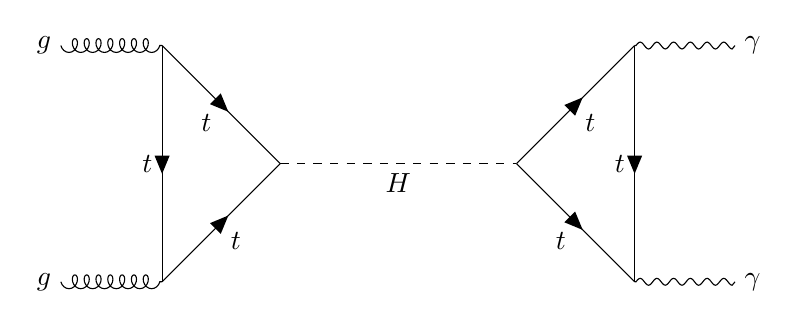
\begin{tikzpicture}[scale=1.5]
\begin{feynman}

\vertex (i1) at (-1,1) {$g$};
\vertex (i2) at (-1,-1) {$g$};

\vertex (a) at (0,1);
\vertex (b) at (0,-1);
\vertex (c) at (1,0);

\vertex (d) at (3,0);
\vertex (e) at (4,1);
\vertex (f) at (4,-1);

\vertex (f1) at (5,1) {$\gamma$};
\vertex (f2) at (5,-1) {$\gamma$};

\diagram*{
  (i1) -- [gluon] (a),
  (i2) -- [gluon] (b),
  (a) -- [fermion, edge label'=\(t\)] (b),
  (a) -- [fermion, edge label'=\(t\)] (c),
  (b) -- [fermion, edge label'=\(t\)] (c),
  
  (c) -- [scalar, edge label'=\(H\)] (d),

  (d) -- [fermion, edge label'=\(t\)] (e),
  (d) -- [fermion, edge label'=\(t\)] (f),
  (e) -- [fermion, edge label'=\(t\)] (f),

  (e) -- [photon] (f1),
  (f) -- [photon] (f2),
};

\end{feynman}
\end{tikzpicture}

\section*{VBS diagrams}

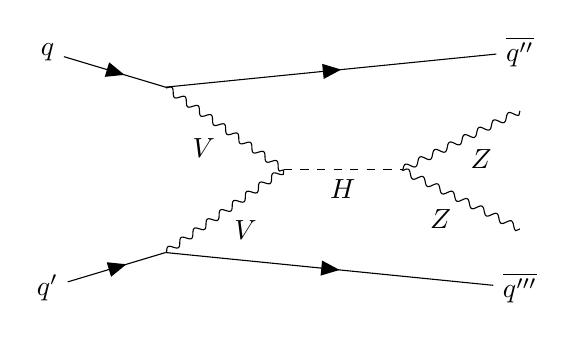
\begin{tikzpicture}[scale=1.5]
\begin{feynman}

\vertex (i1) at (-1,1) {$q$};
\vertex (i2) at (-1,-1) {$q'$};

\vertex (a) at (0,0.7);
\vertex (b) at (0,-0.7);
\vertex (c) at (1,0);

\vertex (d) at (2,0);
\vertex (e) at (3,0.5);
\vertex (f) at (3,-0.5);

\vertex (f1) at (3,1)  {$\overline{q''}$}; 
\vertex (f2) at (3,-1) {$\overline{q'''}$};

\diagram*{
  (i1) -- [fermion] (a),
  (i2) -- [fermion] (b),
  (a) -- [fermion] (f1),
  (b) -- [fermion] (f2),
  
  (a) -- [boson, edge label'=\(V\)] (c),
  (b) -- [boson, edge label'=\(V\)] (c),

  (c) -- [scalar, edge label'=\(H\)] (d),
  
  (d) -- [boson, edge label'=\(Z\)] (e),
  (d) -- [boson, edge label'=\(Z\)] (f),
};

\end{feynman}
\end{tikzpicture}

\section*{VBS diagram: $ZZ \rightarrow 4l$ final state}

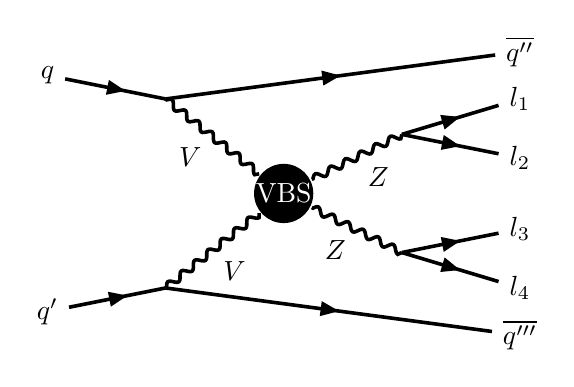
\begin{tikzpicture}[scale=1.5, line width=1.3pt]
\begin{feynman}

\vertex (i1) at (-1,1) {$q$};
\vertex (i2) at (-1,-1) {$q'$};

\vertex (a) at (0,0.8);
\vertex (b) at (0,-0.8);
% Blob
% Interaction blob
\node[
    circle,
    fill=black,
    minimum size=5mm,
    inner sep=0pt
] (v) at (1,0) {\color{white}{VBS}};

\vertex (e) at (2,0.5);
\vertex (f) at (2,-0.5);

\vertex (l1) at (3,0.8) {$l_1$};
\vertex (l2) at (3,0.3) {$l_2$};
\vertex (l3) at (3,-0.3) {$l_3$};
\vertex (l4) at (3,-0.8) {$l_4$};


\vertex (f1) at (3,1.2)  {$\overline{q''}$}; 
\vertex (f2) at (3,-1.2) {$\overline{q'''}$};

\diagram*{
  (i1) -- [fermion] (a),
  (i2) -- [fermion] (b),
  (a) -- [fermion] (f1),
  (b) -- [fermion] (f2),
  
  (a) -- [boson, edge label'=\(V\)] (v),
  (b) -- [boson, edge label'=\(V\)] (v),
   
  
  (v) -- [boson, edge label'=\(Z\)] (e),
  (v) -- [boson, edge label'=\(Z\)] (f),

  (e) -- [fermion] (l1),
  (e) -- [fermion] (l2),
  (f) -- [fermion] (l3),
  (f) -- [fermion] (l4),
};

\end{feynman}
\end{tikzpicture}


\end{document}
